\documentclass{article}
\usepackage{tikz}
\usepackage{amsmath}

\begin{document}

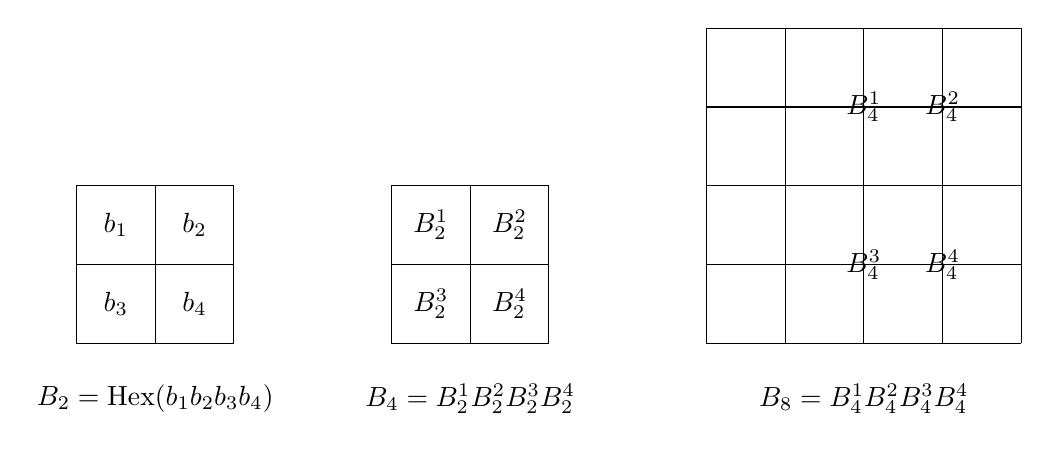
\begin{tikzpicture}

% First small 2x2 grid with b_i
\draw (0,0) grid (2,2);
\node at (0.5,1.5) {$b_1$};
\node at (1.5,1.5) {$b_2$};
\node at (0.5,0.5) {$b_3$};
\node at (1.5,0.5) {$b_4$};

% Label for B_2
\node at (1,-0.7) {$B_2 = \text{Hex}(b_1 b_2 b_3 b_4)$};

% Second 2x2 grid with B_2^i
\draw (4,0) grid (6,2);
\node at (4.5,1.5) {$B_2^1$};
\node at (5.5,1.5) {$B_2^2$};
\node at (4.5,0.5) {$B_2^3$};
\node at (5.5,0.5) {$B_2^4$};

% Label for B_4
\node at (5,-0.7) {$B_4 = B_2^1 B_2^2 B_2^3 B_2^4$};

% Third larger 4x4 grid with B_4^i
\draw (8,0) grid (12,4);
\node at (10,3) {$B_4^1$};
\node at (11,3) {$B_4^2$};
\node at (10,1) {$B_4^3$};
\node at (11,1) {$B_4^4$};

% Label for B_8
\node at (10,-0.7) {$B_8 = B_4^1 B_4^2 B_4^3 B_4^4$};

\end{tikzpicture}

\end{document}